%
\documentclass{beamer}

% Theme choice:
\usetheme{Berkeley}

% Title page details: 
\title{Title: Analyzing Stormwater Best Management Plan Data}
\subtitle{Data encased in lists, wrapped in vectors, swaddled in JSON}
\author{Erik H. Beck}
\institute{USEPA R1}
\date{17 Oct 2023}
% \logo{\large \LaTeX{}}


\begin{document}

% Title page frame
\begin{frame}
    \titlepage 
\end{frame}

% Remove logo from the next slides
% \logo{}


% Outline frame
\begin{frame}{Outline}
    \tableofcontents
\end{frame}



% Cover Photo Frame
\section{Overview}
\begin{frame}{Visualization}
  \begin{figure}
    \centering
       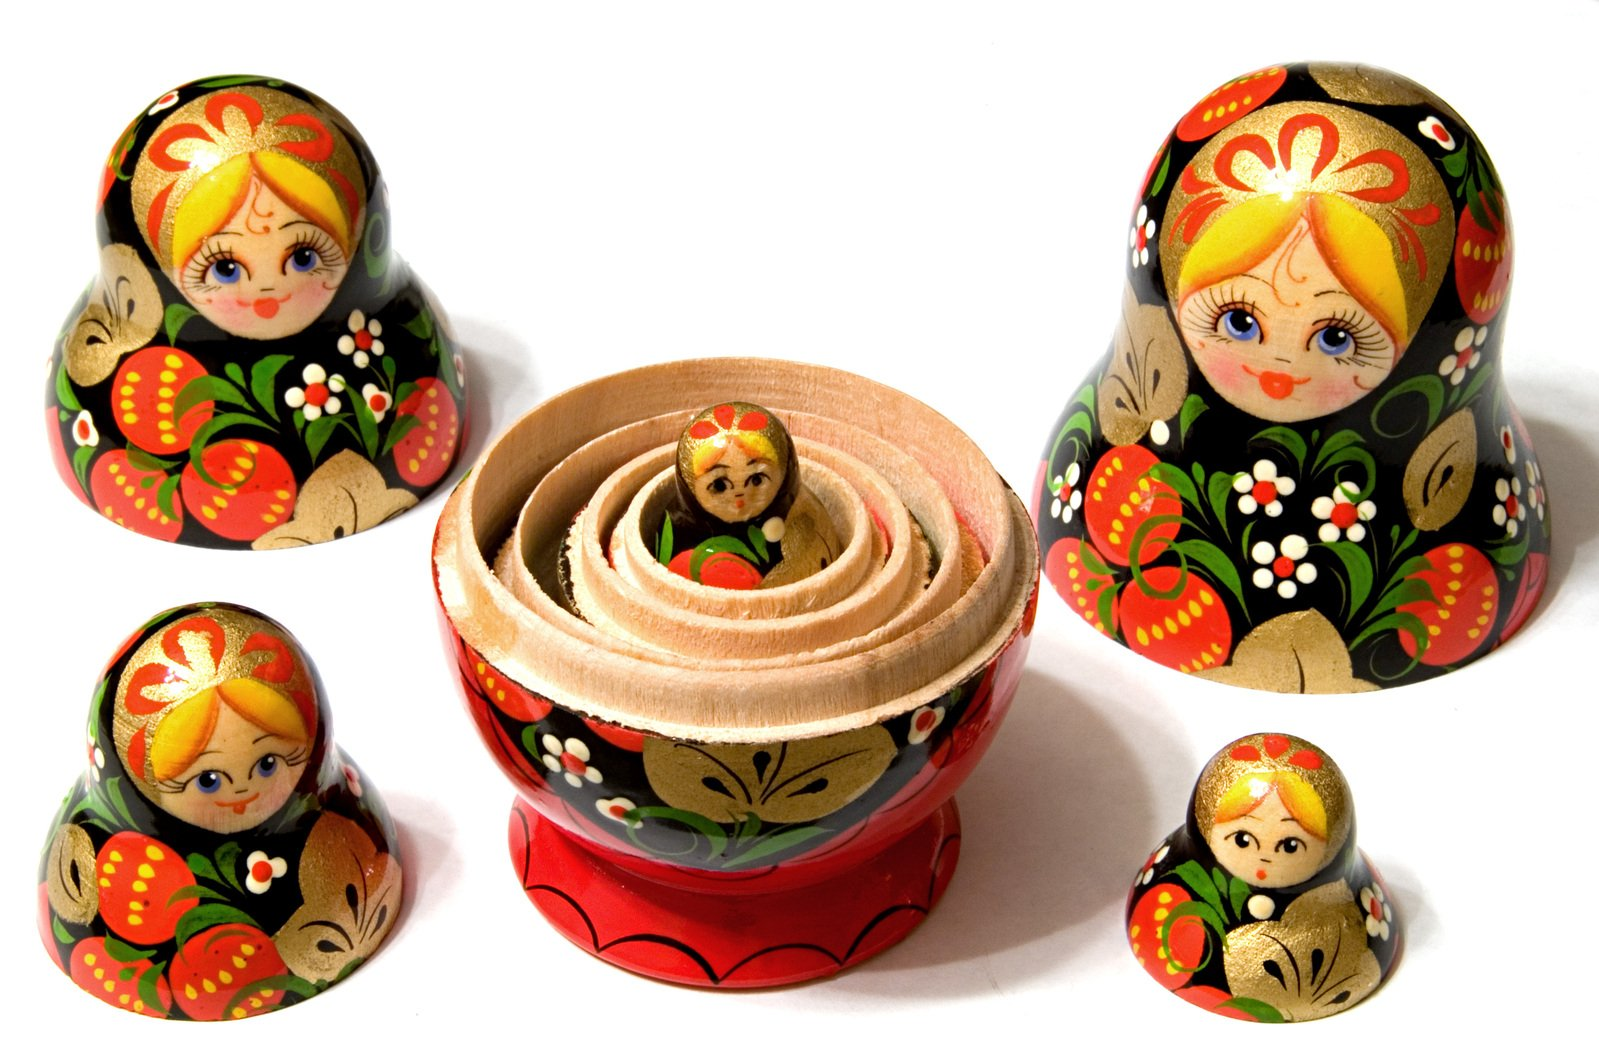
\includegraphics[width=0.50\textwidth]{russian-nesting-doll-1187383.jpg}
       \caption{(https://images.freeimages.com/images/large-previews/6a4/russian-nesting-doll-1187383.jpg)}
  \end{figure}
  Nature of the problem:
  \begin {itemize}
       \item Data encased in lists, wrapped in vectors, swaddled in JSON
  \end{itemize}
\end{frame}

%

\begin{frame}{Speedy Talk: Quick Overview}
  \begin{itemize}
   \item Stormwater::CWA 319::BMPs::GRTS
   \item Q: Why the GRTS System?
   \item A: Strings attached to Govt. money!
   \item Oracle Business Intelligence: Clunky and not very capable
   \item Basic questions to answer:
   \begin{itemize}
        \item What is the mean level of funding for Nonpoint Source
          projects in New England (and the confidence interval)?
	\item How is that funding scattered across appropriation
          years? What does that look like graphically?
	\item Can't answer these basic questions using OBI
   \end{itemize}
  \end{itemize}
\end{frame}

\section{GRTS}

\begin{frame}{Stormwater, CWA 319, Nonpoint Source Pollution, BMPs, and GRTS}
  \begin{itemize}
  \item EPA's GRTS system a required part of getting EPA funding under CWA 319 (NPS)
  \item States have to enter the data on projects using EPA funding 
  \item Entered data is broad info on work done under EPA grants
  \item Data goes into Grants Results and Tracking System (GRTS)
  \item OW/OWOW builds and maintains the system
    \begin{itemize}
    \item Data entered by states, tribes, regions
    \item System can export some data 'natively' to PDF and CSV, but pretty limited
    \end{itemize}
  \end{itemize}
\end{frame}

\section{R}

\begin{frame}{Getting the Data to R}
  \begin{itemize}
  \item OW has developed one Application Programming Interface (API) to GRTS
    \begin{itemize}
	\item Uses HUC12 to find data
	\item One to many relationships of data
	\item One HUC may have zero to many BMP projects associated
           with it across years, grants, etc
        \item More in development
    \end{itemize}
    \item Using the API returns a single JSON structure for a HUC12
    \item JSON is deeply nested; challenge is picking apart the
      material and massaging it for analysis
  \end{itemize}
\end{frame}

\section{Examples}

\begin{frame}[fragile]{Code Fragment}
\begin{verbatim}
HUCmetaData <- function (DataRequestRaw) {
  HUCdataBlobRaw <- DataRequestRaw$content
  HUCdataBlob <- rawToChar(HUCdataBlobRaw)
  HUCdataBlob %>% spread_all -> HUCmetaDataBall
  
  document.id <- HUCmetaDataBall$document.id 
  count <- HUCmetaDataBall$count  
  # The Payload is in 'HUCmetaDataBall$..JSON'. 
  ## Extract elsewhere.
  HUCMetaData <- data.frame (document.id,count) 

  return (HUCMetaData) 
 }

\end{verbatim}
\end{frame}

\begin{frame}{Basic Analysis}
  After the GRTS data is tamed, we can start answering the basic
  questions
 
\end{frame}
\begin{frame}{Question One}
  What's the mean and 'data spread' of GRTS
  funding in New England?
  \begin{figure}
    \centering
    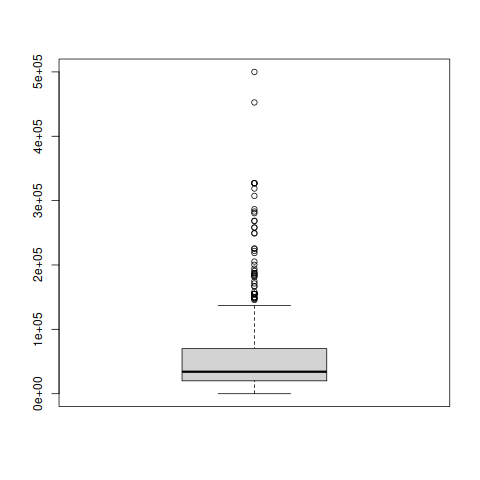
\includegraphics[width=0.50\textwidth]{funds_319.png}
    \caption{USD (\$) for CWA 319 Stormwater BMP Funding in New England}
  \end{figure}
\end{frame}

\begin{frame}{Question Two}
  What does the data look like when grouped by appropriation years?
  \begin{figure}
    \centering
    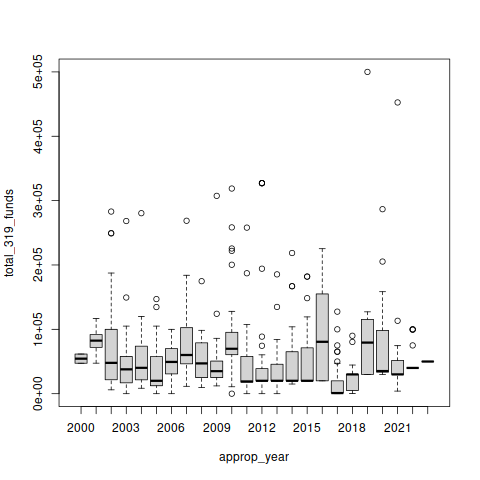
\includegraphics[width=0.50\textwidth]{fundsByAppropYear.png}
    \caption{CWA 319 Stormwater Funding by Federal Fiscal Year in New England}
  \end{figure}
\end{frame}
	 
\section{Wrap-up}

\begin{frame}{Conclusion}
  \begin{itemize}
  \item Using R to analyze GRTS data is very useful
  \item APIs need some work to provide more parts of the dataset
  \item Other APIs in development need to mature and move to the
    production system
  \item Working with the deeply nested JSON data is worth it; trying
    to coerce this info from OBI would be very difficult or
    impossible.
  \end{itemize}
\end{frame}


\begin{frame}{Questions?}
  \centering
  I can take a few questions.
\end{frame}
 
\end{document}
